\documentclass[10pt,a4paper,spanish]{article}

\usepackage[T1]{fontenc} 
\usepackage[utf8]{inputenc}
\usepackage[spanish]{babel}

\usepackage{graphicx}
\usepackage{epstopdf}

\usepackage[export]{adjustbox}
\usepackage{caption}
\usepackage{colortbl} 
\usepackage{dashrule} 
\usepackage{fancyhdr}
\usepackage{float}
\usepackage{framed}
\usepackage[bmargin=2cm,footnotesep=1cm,tmargin=2cm]{geometry} 
\usepackage[pdftex,colorlinks,backref,bookmarks=true,bookmarksnumbered=true,linkcolor=black,urlcolor=black,citecolor=black]{hyperref}
\usepackage[section]{placeins}
\usepackage[labelsep=quad,indention=10pt]{subfig}
\usepackage[spanish,shadow,textsize=small]{todonotes}
\usepackage{wrapfig}
\usepackage{fancyvrb}
\usepackage{xcolor}

% TITULOS
\newcommand{\asig}{Algoritmos y Estructuras de Datos}
\newcommand{\anno}{3º}
\newcommand{\grado}{Grado en Ingeniería Biomédica}
\newcommand{\upm}{Universidad Politécnica de Madrid}
\newcommand{\curso}{}
\newcommand{\ssg}{Rodrigo García Carmona}
\newcommand{\email}{\href{mailto:rodrigo.garciacarmona@ceu.es}{rodrigo.garcia@upm.es}}
\newcommand{\cabecera}[1]{
  \title{Guion de Prácticas}
  \author{\asig\\ \anno\grado\\ \ceu \\ \ssg} 
  \date{#1}
  \maketitle \thispagestyle{fancy}
}

% NUEVAS TODONOTES
\newcommand{\nota}[2][] {\todo[inline, #1]{#2}}
\newcommand{\corregir}[2][] {\todo[color=red, #1]{#2}}
\newcommand{\finaltodo}[2][] {\todo[color=green!40,fancyline #1]{#2}}
\newcommand{\finalnota}[2][] {\todo[color=green!40, inline #1]{#2}}

% PDF
\hypersetup{
  colorlinks=true,
  linkcolor=blue,
  filecolor=magenta,      
  urlcolor=cyan,
  pdfauthor={\ssg},
  pdftitle={Guion de Prácticas},
  pdfsubject={\asig, \grado, \upm, Madrid, España},
  pdfkeywords={algoritmos, estructuras de datos, ingeniería biomédica, guion, prácticas}, 
  pdftoolbar=true,
  pdfmenubar=true,
  pdffitwindow=true,
  pdfnewwindow=true
}

% ENCABEZADO
\pagestyle{fancy}%
  \renewcommand{\headrulewidth}{0.1pt}
  \renewcommand{\footrulewidth}{0.1pt}
  \fancyhf{}
  \fancyhead[L]{
\includegraphics[width=8mm]{templates/ETSIT-UPM.eps}}
  \fancyhead[C]{\small{\asig}\\\small{\grado}}
  \fancyhead[R]{\curso}
  \fancyfoot[L]{}
  \fancyfoot[C]{\thepage}
  \fancyfoot[R]{}

% CAJA SOMBREADA
% comando \sombreado{Título}{Texto}
\definecolor{shadecolor}{rgb}{0.9,0.9,0.9}
\newcommand{\sombreado}[2]{
  \begin{shaded}
    \begin{center} \emph{\textsc{#1}} \end{center}
    \noindent #2\\
  \end{shaded}
}

% CAJA INSTRUCCIONES 
\definecolor{shadecolor}{rgb}{0.9,0.9,0.9}
\newcommand{\instrucciones}[7]{
  \begin{shaded}
    \begin{center} \emph{\textsc{#1}}
    \end{center}
    %\noindent \emph{\textsc{Fecha límite de entrega: }} \emph{#4}\\
    %\emph{\textsc{Peso: }}\emph{#5}\newline\newline
    #6

    #7
  \end{shaded}
}

% Código fuente
\newcommand{\code}[1]{\texttt{#1}}

% Big O
\newcommand{\bigO}{\mathcal{O}}


% Minted
\usepackage{minted}
% Optional: Set a default style. 'manni' is a light, clean style.
% Other popular styles include 'tango', 'monokai', 'solarized-light'.
\usemintedstyle{sas}

% PRACTICA
\newcommand{\practica}{Práctica 4: Concurrencia}
\newcommand{\notaob}{
\begin{center}
Rodrigo García Carmona\\
\href{mailto:rodrigo.garcia@upm.es}{rodrigo.garcia@upm.es}\\
\includegraphics[width=20mm]{templates/by-nc-sa.eps}
\end{center}

Esta práctica es individual y sirve tanto para desarrollar como para poner a prueba los conocimientos adquiridos. Realizar esta práctica es recomendable para aumentar las probabilidades de éxito en los exámenes teóricos.
}

% MACROS

% CONTENIDO
\begin{document}

\instrucciones{\practica}{\tiempo}{\obligatoria}{\fecha}{\peso}{\notaob}

\section{Preparación de la práctica}
\label{sec:previa}

El objetivo de esta práctica es aprender a utilizar hebras (\textit{threads}) para implementar programas que hagan uso de la concurrencia. Se estudiarán los siguientes conceptos:

\begin{itemize}
    \item Implementación de hebras.
    \item Arranque, parada y sincronización de hebras.
    \item Uso de la concurrencia para implementar simulaciones.
    \item Uso de la concurrencia para paralelizar trabajos usando tareas.
\end{itemize}

\sombreado{Trabajo previo al laboratorio}{El tiempo de las clases de laboratorio es muy valioso, ya que en ellas tendrá a su disposición a los profesores para resolver cualquier duda que le pueda surgir. Por tanto, para facilitar al máximo el aprovechamiento de este tiempo, las prácticas se han dividido en varias secciones. La primera de ellas (``preparación de la práctica'') puede ¡y debe! realizarse \textbf{antes de la sesión de laboratorio} propiamente dicha. Leer esta sección antes de entrar a clase hará que su tiempo en el laboratorio sea más productivo y provocará que las dudas más importantes le surjan \textbf{durante la clase}, y \textbf{no después}, cuando se encuentre estudiando solo en su casa y la única opción que le quede sea escribir un email al profesor.

De hecho, es especialmente importante evitar que se den situaciones como esta la noche antes de un examen.}

\subsection{Sistemas simples y complejos}

Existen, a grandes rasgos, dos tipos de sistemas en lo que a la capacidad para modelarlos y calcular qué resultado van a producir respecta:

\begin{itemize}
    \item Los \textbf{sistemas simples}, caracterizados por un comportamiento predecible, pues está basado en un conjunto de reglas. Su resultado puede calcularse recurriendo a la aplicación de estas reglas sobre las condiciones iniciales en las que se encuentra el sistema.
    \item Los \textbf{sistemas complejos}, compuestos de varios componentes que, al interactuar entre sí, producen comportamientos de un orden superior. La principal característica de los sistemas complejos es que no es posible predecir estos comportamientos a partir de las características individuales de los componentes que los producen.
\end{itemize}

\subsubsection{Sistemas simples}

Los sistemas simples son la piedra angular de la física clásica y la ingeniería tradicional, en la que los problemas se descomponen en partes más pequeñas, que son resueltas de forma independiente. Se caracterizan por su predictibilidad y su dependencia de un conjunto finito y conocido de reglas y condiciones iniciales. Poseen las siguientes características:

\begin{itemize}
    \item \textbf{Solución analítica:} El comportamiento de un sistema simple está descrito por completo mediante una fórmula o un conjunto de ecuaciones con una solución analítica. Si se conocen las condiciones iniciales, el estado futuro del sistema puede calcularse sustituyendo las variables de las ecuaciones por estas condiciones iniciales.
    \item \textbf{Linealidad o no linealidad limitada:} En los sistemas simples, un cambio en las condiciones iniciales produce un cambio similar en el resultado.
    \item \textbf{Predictibilidad a largo plazo:} Calcular el estado de un sistema simple a largo plazo no es sustancialmente más difícil que hacerlo a corto plazo. Muchas veces, es algo tan sencillo como cambiar el valor de la variable que representa el tiempo.
    \item \textbf{Reduccionismo:} El reduccionismo es una estrategia que permite calcular el comportamiento de un ``todo'' a través de la suma de los comportamientos de sus partes. Los sistemas simples son reduccionistas en tanto en cuanto basta con entender qué hacen cada una de sus partes constituyentes para entender el sistema en su conjunto.
\end{itemize}

Un ejemplo típico de un sistema simple es la trayectoria de un proyectil: una vez se conocen la masa, la velocidad inicial y las fuerzas aplicadas, su posición en cualquier momento del futuro es perfectamente calculable mediante la aplicación de un conjunto de ecuaciones.

En los sistemas simples, \textbf{la simulación no es una necesidad}, sino una herramienta de conveniencia. En el ejemplo del proyectil, una simulación podría usarse para visualizar la trayectoria o para calcular soluciones intermedias, pero no es la única vía para obtener el resultado (qué posición ocupa el proyectil al final de su trayectoria y cuándo la alcanza).

\subsubsection{Sistemas complejos}

Los sistemas complejos están formados por agentes o elementos (los componentes del sistema) que actúan o reaccionan de forma independiente, cada uno obedeciendo sus propias reglas. De las relaciones entre agentes y las interacciones entre ellos surgen una serie de efectos (el resultado del sistema). Los sistemas complejos están cada vez más presentes en la ingeniería y aparecen constantemente en las ciencias, especialmente en las de la vida.

El comportamiento de los sistemas complejos es inherentemente difícil de modelar, debido a las interacciones entre los componentes que los integran. Poseen las siguientes características:

\begin{itemize}
    \item \textbf{Múltiples agentes concurrentes:} El sistema se compone de un gran número de agentes que operan en paralelo, es decir, de forma concurrente. Cada agente obedece sus propias reglas, que pueden ser más o menos sencillas.
    \item \textbf{No linealidad:} Debido a fenómenos como los bucles de realimentación (entre otros), los sistemas complejos tienden a producir resultados muy diferentes frente a pequeños cambios en las condiciones iniciales.
    \item \textbf{Dependencia de la secuencia de interacciones:} El estado futuro de un sistema complejo no puede predecirse únicamente a partir del estado actual, sino que también se necesita conocer los pasos intermedios entre el actual y el que se desea conocer.
    \item \textbf{Comportamiento emergente:} Los sistemas complejos exhiben un ``patrón global'' que surge espontáneamente de las interacciones locales. Este comportamiento, si bien no está expresado de forma explícita en ninguna parte concreta del sistema es, sin embargo, indudablemente real. Además, este patrón global no puede predecirse mediante una simple agregación del comportamiento de las partes. 
\end{itemize}

\sombreado{Complejo no es lo mismo que complicado}{Los sistemas simples pueden ser muy complicados (las fórmulas que los regulan son difíciles de calcular o tienen muchas variables), pero eso no hace que sean complejos; ningún comportamiento emerge de ellos. De la misma forma, los sistemas complejos pueden ser sencillos (cada agente, individualmente, se comportan siguiendo unas reglas que pueden ser elementales), pero eso no hace que sean simples.}

Este conjunto de características nos lleva a un conclusión sumamente importante: en cuanto el número de agentes o componentes de un sistema complejo crece a partir de cierto punto, es matemáticamente imposible escribir una fórmula cerrada que describa el estado del sistema a largo plazo.

Además, los sistemas complejos exhiben una dependencia extrema a las condiciones iniciales: un cambio minúsculo en una condición inicial, al propagarse a través de las interacciones concurrentes de los agentes, se amplifica hasta producir resultados completamente diferentes. Este fenómeno es conocido popularmente como el ``efecto mariposa''.

Existen numerosos ejemplos de sistemas complejos, que van desde lo más pequeño (una célula) hasta lo más grande (el clima o el ecosistema). En todos ellos existe indudablemente un comportamiento global que es, a la vez, irreductible. Si piensa en  el desplazamiento de una bandada de pájaros, en la congestión en el transporte público de una ciudad o en el metabolismo humano, será capaz de reconocer patrones globales. En todos estos ejemplos, una predicción a largo plazo es imposible sin una simulación que, en muchos casos, deberá incluso ejecutarse múltiples veces con pequeñas variaciones para entender el abanico de resultados posibles.

Un ejemplo muy sencillo de enteder (y a la vez sorprendentemente divertido) de todo esto es el \href{https://es.wikipedia.org/wiki/Juego_de_la_vida}{Juego de la Vida de Conway}, en el que un conjunto de reglas sencillas generan patrones que se ``autoreplican'' y se ``desplazan''. Un ejemplo de patrón puede verse en la Figura \ref{fig:gameoflife}.

\begin{figure}[!htbp]
  \centering
  
\includegraphics[width=\textwidth]{files/GameOfLife.png}
  \caption{Patrón ``Gosper glider gun'' en el Juego de la Vida de Conway.}
  \label{fig:gameoflife}
\end{figure}

De hecho, para algunos autores, el universo en su conjunto no es sino un gran sistema complejo, del que todos formamos parte.

\sombreado{Vamos a ponernos profundos}{La existencia de la complejidad emergente plantea preguntas sumamente profundas sobre dos problemas filosóficos: la consciencia y el libre albedrío.

Y es que quizá la consciencia (la capacidad de experimentar el universo) y el libre albedrío (la capacidad para tomar decisiones intencionalmente) no sean sino comportamientos emergentes que aparecen en uno de los sistemas complejos más grandes que conocemos: el cerebro humano, compuesto por miles de millones de neuronas. Esto es lo que postulan varias teorías de la consciencia, siendo la más popular (aunque no la única) la \href{https://iep.utm.edu/integrated-information-theory-of-consciousness/}{Teoría de la Información Integrada}. 

Desde esta perspectiva, el libre albedrío no sería una fuerza que rompe las leyes de la física, sino un fenómeno emergente a un nivel de complejidad tan alto que las interacciones no lineales y la sensibilidad a las condiciones iniciales hacen que el comportamiento del sistema sea impredecible. Y aquí se está usando la palabra ``impredecible'' con el significado completo y literal de la misma. Es decir no es que el conjunto de decisiones que toma un humano sea \textbf{impredecible en la práctica} debido a que hay variables ocultas o mecanismos desconocidos, sino que es \textbf{realmente impredecible}: solo una ``ejecución'' completa del sistema complejo (es decir, la vida de la propia persona) podría llegar al mismo resultado. Esta teoría podría interpretarse, desde un punto de vista religioso, como que ni siquiera un Dios omnisciente sería capaz de conocer el destino de una persona sin antes ``instanciarla''.

No obstante, para que esta interpretación sea factible, la propia causalidad debe de ser en sí misma uno de los fenómenos emergentes de un sistema complejo, algo que el neurocientífico Erik Hoel parece haber demostrado \href{https://arxiv.org/abs/2503.13395}{en un artículo publicado en 2025}. Si desea profundizar más en esto, le recomiendo la lectura de \href{https://www.theintrinsicperspective.com/p/i-figured-out-how-to-engineer-emergence}{este resumen del artículo}, muy fácil de entender.}

\subsection{Simulación de sistemas complejos}

De lo explicado hasta ahora se puede concluir que la única forma de predecir el resultado de un sistema complejo es ejecutar una simulación lo más fidedigna posible del mismo. Esta simulación deberá instanciar a tantos agentes como posea el sistema complejo, dejando que estos se comporten de forma independiente, obedeciendo cada uno las reglas que lo gobiernan.

Y esto es, precisamente, lo que nos permite hacer la programación concurrente. En ella, cada una de las hebras representará a un agente, que se ejecutará por su cuenta e interactuará con el resto del sistema. Si el sistema ha sido modelado correctamente, esta técnica suele arrojar predicciones muy fidedignas, convirtiéndose en una herramienta de predicción y análisis excelente.

\subsection{Modelado del servicio de Urgencias de un hospital}

El servicio de Urgencias de un hospital es un sistema complejo paradigmático, pues posee:

\begin{itemize}
    \item \textbf{Agentes independientes:} Médicos, enfermeros, pacientes, equipos de observación, personal de triaje...
    \item \textbf{Interacciones no lineales:} La llegada de un paciente crítico (una perturbación pequeña) consume múltiples recursos simultáneamente (un médico, un equipo, una sala) durante un tiempo impredecible.
    \item \textbf{Emergencia:} El tiempo de espera promedio, la ocupación de camas y la saturación del personal son propiedades emergentes que no se pueden calcular directamente, sino que surgen de la simulación de las interacciones concurrentes minuto a minuto.
\end{itemize}

\begin{figure}[!htbp]
  \centering
  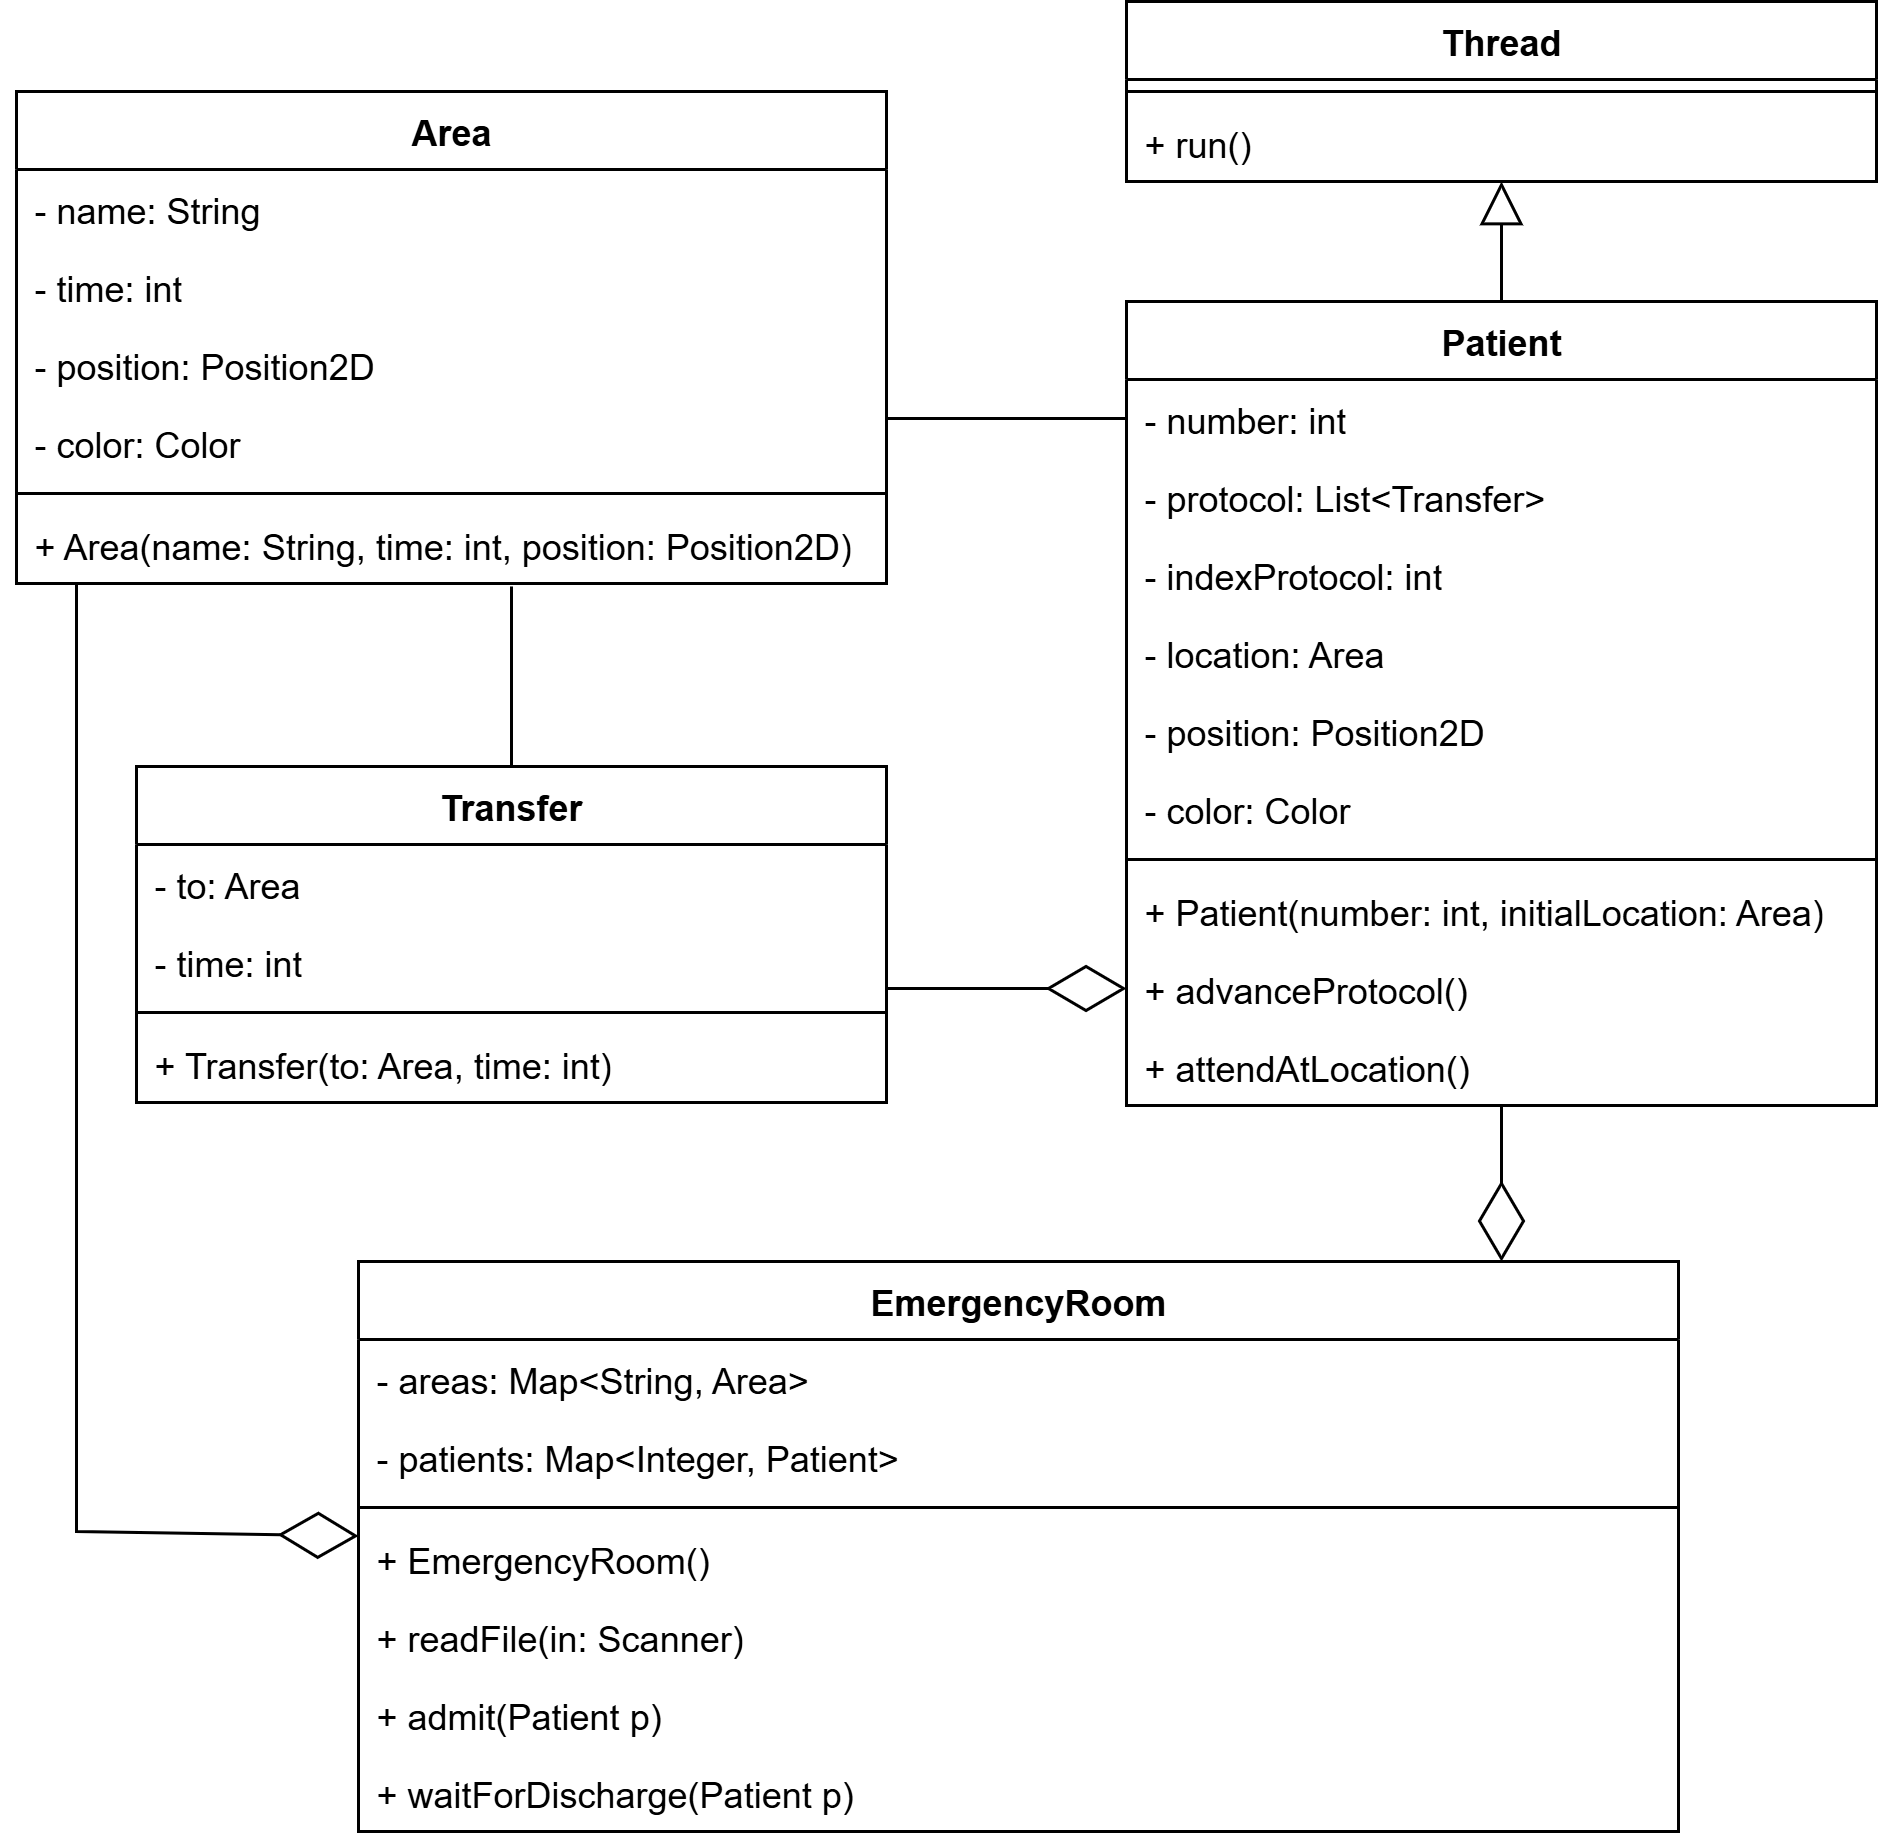
\includegraphics[width=0.95\textwidth]{files/ALED4-DataModel.png}
  \caption{Diagrama de clases del simulador del servicio de Urgencias.}
  \label{fig:dataModel}
\end{figure}

En la \textbf{primera parte} (¡ojo, hay dos!) de esta práctica se va a modelar un servicio de Urgencias simplificado, con las clases que aparecen en la Figura \ref{fig:dataModel}. En el diagrama se han omitido, por claridad, los métodos \code{getX()}, \code{setX()}, \code{equals()} y \code{toString()} de cada clase.

Vamos a analizar una por una las clases del diagrama, para explicar su propósito:

\begin{itemize}
    \item \code{Area} representa cada una de las secciones del servicio de Urgencias del hospital. Tiene dos atributos que afectan a la simulación: \code{name}, el nombre de la sección; y \code{time}, que es el tiempo que tardará en ser atendido (en milisegundos) un paciente. Los otros dos atributos restantes (\code{position} y \code{color}) solo afectan a la forma en la que la sección será representada por la interfaz gráfica, y no deberá preocuparse de ellos.
    \item \code{Transfer} modela el desplazamiento de un paciente hasta una sección distinta a aquella en la que se encuentra. Posee dos atributos: \code{to}, que indica el \code{Area} hacia la que se mueve el paciente; y \code{time}, que es el tiempo (en milisegundos) que llevará este movimiento.
    \item \code{Patient} es la clase que encapsula el comportamiento de un paciente individual. Cada paciente está identificado por un \code{number}, que será un código único, para preservar su anonimato. Además también posee el atributo \code{location}, que representa el \code{Area} en la que se encuentra el paciente en el momento actual y que deberá estar siempre actualizado.

    Todo paciente tiene también un \code{protocol}, que no es más que una \code{List} ordenada de \code{Transfers} que modela el recorrido que seguirá dicho paciente por el servicio de Urgencias según vaya avanzando el tiempo. Para saber en qué punto del protocolo se encuentra el paciente en un momento dado se utiliza el atributo \code{indexProtocol}, que empieza valiendo 0 cuando el \code{Patient} es creado.

    Como en el caso de \code{Area}, \code{Patient} también cuenta con los atributos \code{position} y \code{color}, que no afectan a la simulación; solo son utilizados por la interfaz gráfica.

    Fíjese además en que la clase \code{Patient} también tiene dos métodos:
    \begin{itemize}
        \item \code{advanceProtocol()}, que hace que el paciente avance al siguiente paso en el protocolo.
        \item \code{attendAtLocation()}, que hace que el paciente espere en el \code{Area} en la que se encuentra el tiempo que esta última determine.
    \end{itemize}
    \item Por último, la clase \code{EmergencyRoom} representa el servicio de Urgencias en su conjunto. Como tal, cuenta con un registro de \code{areas} y \code{patients} (\code{Maps} en los que las claves son el nombre de cada \code{Area} y el número de cada \code{Patient}, según corresponda), así como los siguientes métodos:
    \begin{itemize}
        \item \code{readFile(Scanner in)}, que se usa para cargar la información del servicio (pacientes incluídos) a partir de un fichero.
        \item \code{admit(Patient p)}, que sirve para empezar a atender al \code{Patient} que se pasa como argumento.
        \item \code{waitForDischarge(Patient p)}, que espera hasta que el \code{Patient} recibido termine su protocolo.
    \end{itemize}
\end{itemize}

Estas clases se encuentran en el paquete \code{es.upm.dit.aled.lab4.er}. Dedique un tiempo a leerlas y entender como funcionan.

\textbf{Responda a las siguientes preguntas:}

\begin{itemize}
    \item En el diagrama, ¿qué significa la flecha que va desde \code{Patient} hasta \code{Thread}?
    \item ¿Qué metodo de la clase \code{Patient} no aparece dentro de dicha clase en el diagrama (aparte de \code{getX()}, \code{setX()}, \code{equals()} y \code{toString()})? ¿Para qué sirve dicho método? ¿A qué clase pertenece?
    \item En esta simulación simplificada de un servicio de Urgencias, ¿los objetos de qué clase se ejecutarán de forma concurrente? ¿Por tanto, qué agentes existen en esta simulación?
\end{itemize}

\subsection{Lectura de archivos y lanzamiento de la simulación}
\label{sec:archivo}

Ahora fíjese en el archivo \code{er\_data.txt}, que se encuentra en la carpeta \code{er}. Este archivo contiene la información necesaria para simular un servicio de Urgencias concreto. En él aparecen varias secciones:

\begin{verbatim}
AREA  80  80 1000 Admision
AREA 160 300 1000 Triaje
AREA 160 190 1000 SalaEspera
AREA 320  80 1000 Box_Trauma
...
\end{verbatim}

Así como pacientes y sus protocolos:

\begin{verbatim}
...
PATIENT 1 Admision
TRANSFER 1 Triaje 3000
TRANSFER 1 SalaEspera 3000
TRANSFER 1 Box_Trauma 3000
TRANSFER 1 SalaEspera 3000
TRANSFER 1 Box_Trauma_Final 3000
...
\end{verbatim}

Observe el código del método \code{readFile(Scanner in)} de la clase \code{EmergencyRoom}, que es el que procesa estos archivos.

\textbf{Responda a las siguientes preguntas:}

\begin{itemize}
    \item ¿En las líneas que empiezan por la palabra ``AREA'', qué significan cada uno de los números y el texto que la siguen?
    \item ¿En las líneas que empiezan por la palabra ``PATIENT'', qué significan el número y el texto que la siguen?
    \item ¿En las líneas que empiezan por la palabra ``TRANSFER'', qué significan los dos números y el texto que la siguen?
\end{itemize}

\subsection{Interfaz gráfica}

Dentro del paquete \code{es.upm.dit.aled.lab4.er.gui} se encuentran las clases necesarias para ejecutar una interfaz gráfica que permite visualizar el movimiento de los pacientes por el servicio de Urgencias. Estas clases son:

\begin{itemize}
    \item \code{Position2D}, que simplemente encapsula las coordenadas $x$ e $y$, necesarias para representar un punto en un espacio bidimensional.
    \item \code{EmergencyRoomGUI}, que crea una ventana y dibuja dentro de ella cajas para representar las secciones y puntos para representar a los pacientes. Aunque no es necesario que entienda cómo está implementado este código, sí que es importante que se fije en la existencia de tres métodos, pues tendrá que utilizarlos durante la práctica:

    \begin{itemize}
        \item \code{getInstance()}: Este método \textbf{estático} devuelve la referencia a un objeto de la clase \code{EmergencyRoomGUI}, que necesitará para ejecutar los dos métodos \textbf{no estáticos} que aparecen a continuación.
        \item \code{animateTransfer(Patient p, Transfer t)}: Este método ejecuta la animación que mueve al \code{Patient} proporcionado desde su ubicación actual (\code{location}) hasta el  destino del \code{Transfer} (\code{to}). \textbf{Tarda en ejecutarse tanto como dure el traslado.}
        \item \code{removePatient(Patient p)}: Este método borra al \code{Patient} proporcionado de la pantalla, y debe ser invocado cuando un paciente ha terminado su protocolo. 
    \end{itemize}
\end{itemize}

Sirva de ejemplo del uso de estos métodos la siguiente línea de código, que ejecuta la animación de un paciente:

\begin{minted}[
  frame=lines, % Adds a frame around the code
  framesep=2mm,
  % linenos % Enables line numbers
]{java}
    EmergencyRoomGUI.getInstance().animateTransfer(patient, transfer);
\end{minted}

\sombreado{Patrón singleton}{Quizá se esté preguntando por qué demonios tiene que usar el método \code{getInstance()} en lugar de un constructor para obtener la referencia a un objeto \code{EmergencyRoomGUI}. De hecho, ¡el constructor de \code{EmergencyRoomGUI} es privado! ¡Qué locura es esta!

Pues bien, esta forma de estructurar una clase (constructor privado y métodos \code{initialize()} y \code{getInstance()}) es típica de un patrón de diseño (una forma de estructurar programas) que recibe el nombre de \textit{singleton}. Se usa, como su nombre sugiere, cuando queremos que solo sea posible crear una única instancia de una clase, que debe ser compartida por todos los que quieran usarla. En este caso, se ha hecho así porque siempre vamos a tener una única interfaz gráfica para la simulación. Ni más, ni menos.}

\subsection{Objetivo y descarga de la práctica}

Este práctica, a diferencia de las anteriores, tiene dos objetivos:

\begin{itemize}
    \item El primero, que ya conoce, es la simulación de un servicio de Urgencias de un hospital usando concurrencia. Esta parte de la práctica se desarrolla en la Sección \ref{sec:simulacion}.
    \item El segundo es la aceleración del algoritmo de búsqueda lineal de cadenas de nucleótidos en un genoma que desarrolló en la práctica 3. Esta aceleración será posible gracias a la ejecución en paralelo, usando tantas hebras como procesadores tenga su ordenador. Esta parte de la práctica se desarrolla en la Sección \ref{sec:paralelizacion}.
\end{itemize}

Sí, esta práctica es un poco más larga de lo normal. Pero, a cambio, la siguiente (la práctica 5) será un poco más corta. Se lo prometo.

La práctica está disponible en GitHub, en la siguiente dirección de Internet (URI):

\href{https://github.com/rgarciacarmona/ALED-lab4}{https://github.com/rgarciacarmona/ALED-lab4}

Recuerde que, para poder importar el repositorio en Eclipse debe seleccionar \textit{File $\to$ Import...} y, de entre las opciones disponibles, \textit{Git $\to$ Projects from Git $\to$ Clone URI}. A continuación le aparecerá un menú en el que tendrá que introducir la URI que aparece en el párrafo anterior.

Una vez descargado el código de la práctica, verá que este está compuesto únicamente de dos paquetes (uno de ellos con, a su vez, un subpaquete):

\begin{itemize}
    \item \code{es.upm.dit.aled.lab4.er}: Que corresponde a la primera parte de la práctica.
    \item \code{es.upm.dit.aled.lab4.genome}: Que corresponde a la segunda parte de la práctica.
\end{itemize}

Enhorabuena, ya ha terminado con el trabajo previo a la sesión de laboratorio. Las secciones de la \ref{sec:laboratorio} en adelante puede realizarlas en clase.

\section{Simulación de un servicio de Urgencias}
\label{sec:laboratorio}
\label{sec:simulacion}

En esta primera parte de la práctica, terminará de implementar el código de un simulador del servicio de Urgencias de un hospital. Como ya se habrá percatado al contestar las preguntas de la Sección \ref{sec:previa}, este es un sistema complejo que emerge de la interacción de varios agentes: los pacientes.

Antes de continuar, repase de nuevo el diagrama que aparece en la Figura \ref{fig:dataModel}, que contiene las clases del paquete \code{es.upm.dit.aled.lab4.er} que modelan el servicio de Urgencias. Es bueno que las tenga frescas en la cabeza.

\subsection{Ejecución de la simulación}

Para lanzar la simulación, deberá ejecutar el método \code{main()} de la clase \code{Simulation}. Este método crea una nueva instancia de \code{Simulation}, pasándole como parámetro el primer argumento que recibe el programa al ejecutarse. Inmediatamente después, llama al método \code{start()} del objeto de \code{Simulation} que acaba de crear.

Fíjese en el código del constructor de \code{Simulation}:

\begin{minted}[
  frame=lines, % Adds a frame around the code
  framesep=2mm,
  % linenos % Enables line numbers
]{java}
/**
 * Simulates an emergency room from a provided file
 */
public Simulation(String file) throws FileNotFoundException {
    // Initializes EmergencyRoom
    this.er = new EmergencyRoom();
    // Loads data from file
    File inputFile = new File(file);
    er.readFile(new Scanner(inputFile));
    // Initializes the GUI
    EmergencyRoomGUI.initialize(er);
}
\end{minted}

\textbf{Responda a la siguiente pregunta:}

\begin{itemize}
    \item ¿Cuál debe ser el primer argumento del programa si queremos que se ejecute el servicio de Urgencias que se describe en la Sección \ref{sec:archivo}?
\end{itemize}

A continuación, cree una configuración de lanzamiento que tenga como resultado la ejecución del servicio descrito en la Sección \ref{sec:archivo} y ejecútela.

Debería ver algo muy similar a la pantalla que aparece en la Figura \ref{fig:emptySimulation}.

\begin{figure}[!htbp]
  \centering
  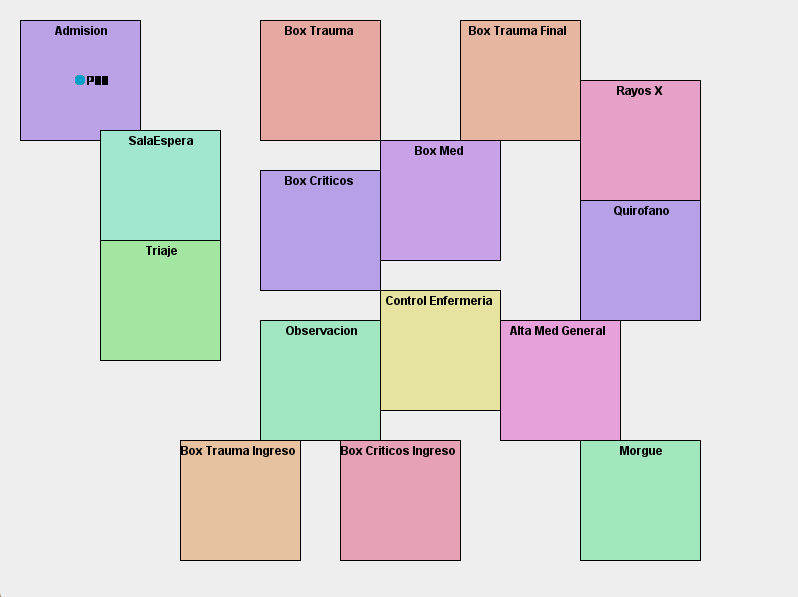
\includegraphics[width=0.9\textwidth]{files/emptySimulation.png}
  \caption{Simulación del servicio de Urgencias.}
  \label{fig:emptySimulation}
\end{figure}

Como puede observar, más allá de mostrar las secciones del servicio y a todos los pacientes en Admisión, no ocurre nada. Esto se debe a que dos de las clases, \code{Patient} y \code{EmergencyRoom} aún tienen métodos sin implementar. Le toca a usted encargarse de ello.

\subsection{Implementación de la clase \code{Patient}}

\code{Patient} modela a los pacientes del hospital, que pueden realizar dos ``acciones'':

\begin{itemize}
    \item \textbf{Ser atendidos en la ubicación en la que se encuentran:} Este comportamiento se produce en el interior del método \code{attendedAtLocation()}, y es muy sencillo: el paciente simplemente tiene que esperar el tiempo correspondiente al \code{Area} en la que se encuentre en ese momento.
    \item \textbf{Avanzar al siguiente paso en su protocolo:} Este comportamiento se produce en el interior del método \code{advanceProtocol()}. Se compone de los siguientes pasos:

    \begin{enumerate}
        \item Pedir a la interfaz gráfica \code{EmergencyRoomGUI} que ejecute una animación que lleve el punto que representa al paciente hasta su nueva ubicación.
        \item Cambiar la ubicación actual del paciente.
        \item Avanzar el protocolo hasta el siguiente paso.
    \end{enumerate}

    Tenga en cuenta que este método, a diferencia de \code{attendedAtLocation()} \textbf{no debe esperar}; la espera ya la realiza \code{EmergencyRoomGUI} al ejecutar la animación.
\end{itemize}

Implemente estos dos métodos.

\sombreado{Trazas}{Para facilitarle la tarea de arreglar los errores que, inevitablemente, tendrá su código, considere hacer que los pacientes impriman por pantalla su número y el comportamiento que están ejecutando en un momento dado. Créame, cuando tenga 20 pacientes interactuando a la vez lo va a agradecer.}

\code{Patient} extiende la clase \code{Thread}, por lo que también deberá implementar el método \code{run()}. Este método es el que se ejecuta cuando alguien arranca las hebras de los pacientes y, por tanto, deberá utilizar los métodos que acaba de programar para representar el comportamiento de un paciente, que será el siguiente:

\begin{enumerate}
    \item Ser atendido en la ubicación actual.
    \item Avanzar al siguiente paso en su protocolo.
    \item Vuelta al punto 1.
\end{enumerate}

Este proceso termina cuando se ha llegado al último paso del protocolo. Tras ser atendido en esta última localización, el paciente deberá pedir a \code{EmergencyRoomGUI} que lo elimine, para que el punto que representa al paciente desaparezca de la pantalla.

\subsection{Implementación de la clase \code{EmergencyRoom}}

Ahora que ha terminado de implementar los pacientes, ha llegado el momento de que alguna parte del programa los maneje como los \code{Threads} que son. Y esa parte es \code{EmergencyRoom}. En esta clase hay dos métodos que deberá implementar:

\begin{itemize}
    \item \code{admit(Patient patient)}, que comienza la ejecución del \code{Patient} que se le pasa como parámetro.
    \item \code{waitForDischarge(Patient patient)}, que se queda esperando a que el \code{Patient} que se le pasa como parámetro finalice.
\end{itemize}

Cuando termine, ejecute de nuevo la simulación. Si lo ha hecho todo correctamente, podré contemplar como dos decenas de pacientes campan a sus anchas por el servicio de Urgencias.

Enhorabuena, ha terminado la \textbf{primera parte} de la práctica. Tómese un breve descanso y a por la segunda parte.

\section{Aceleración de un algoritmo de búsqueda en un genoma}
\label{sec:paralelizacion}

La concurrencia no solo es útil para la simulación de sistemas complejos, sino también para aprovechar el paralelismo inherente a las arquitecturas \textit{hardware} de los ordenadores actuales, pudiendo así resolver ciertos problemas computacionales en un tiempo menor.

Para ilustrar esto, en la \textbf{segunda parte} de esta práctica va a reimplementar el algoritmo que desarrolló en la Sección 2 de la práctica 3. Así que, antes de nada, abra dicha práctica y repase tanto el enunciado como el código que programó usted mismo (esperemos).

La idea es crear una nueva versión de su búsqueda lineal, de tal manera que se lancen tantas tareas (hebras que devuelven un resultado) como procesadores (o núcleos) posea el equipo en el que está trabajando, dividiéndose el espacio de búsqueda de forma equitativa entre ellas. Si, por ejemplo, su ordenador dispone de 8 procesadores, el programa resultante lanzará 8 tareas, encargándose cada una de las cuales de buscar en una octava parte del genoma. En el ejemplo, esta estrategia debería lograr que el tiempo de búsqueda se reduzca a aproximadamente una octava parte del original.

Fíjese en las clases del paquete \code{es.upm.dit.aled.lab4.genome}:

\begin{itemize}
    \item \code{FASTAException}: una clase hija de \code{Exception} cuyo propósito es identificar que una excepción tiene su origen en el procesado de los datos obtenidos a partir de un archivo FASTA. Esta clase \textbf{no cambia respecto a la práctica 3}.
    \item \code{FASTASearchCallable}: una clase que ejecutará la búsqueda lineal (como en la práctica 3), pero que trabajará sobre un fragmento del genoma en lugar de sobre su totalidad. Esta clase contendrá el código equivalente a los métodos \code{search()} y \code{compare()} de la práctica 3. Además, esta clase implementa el interfaz \code{Callable}, ya que es una tarea que debe poder ser lanzada como hebra.
    \item \code{FASTAReaderThreads}: una clase que ejecutará tantas tareas \code{FASTASearchCallable} como procesadores tenga el equipo, indicando a cada una sobre qué parte del genoma debe buscar. Según estas vayan terminando, \code{FASTAReaderThreads} irá agregando los resultados en un único conjunto, que será el que devuelva. Esta clase reutiliza gran parte del código de la clase \code{FASTASearch} de la práctica 3 (todo menos los métodos \code{search()} y \code{compare()}.
\end{itemize}

\subsection{Implementación de la clase \code{FASTASearchCallable}}

La clase \code{FASTASearchCallable} lleva a cabo una búsqueda lineal dentro de un rango \code{[lo,hi)} del array de bytes del genoma (\code{content} en \code{FASTAReaderThreads}). Por tanto, el constructor de \code{FASTASearchCallable} tendrá el siguiente aspecto:

\begin{minted}[
  frame=lines, % Adds a frame around the code
  framesep=2mm,
  % linenos % Enables line numbers
]{java}
/**
 * Creates a new FASTASearchCallable that performs a linear search inside the
 * [lo, hi) range of the genome.
 * 
 * @param reader  FASTAReaderThreads that contains the genome (content) and how
 *                many bytes (validBytes) of this content are valid. Usually
 *                the one that has called this constructor.
 * @param lo      The lower bound of the segment of content to be searched.
 * @param hi      The higher bound of the segment of content to be searched.
 * @param pattern The pattern to be found.
 */
public FASTASearchCallable(FASTAReaderThreads reader,
                    int lo, int hi, byte[] pattern) {
    // TODO
}
\end{minted}

Implemente este constructor. Al hacerlo, sea consciente de que la razón de que se le pase una referencia a \code{FASTAReaderThreads} es porque el método \code{compare()} necesita acceder al contenido del genoma mediante el método \code{getContent()} de \code{FASTAReaderThreads}.

\sombreado{Copia de arrays}{Al constructor de \code{FASTAReaderThreads} no se le pasa una copia de su sección del genoma, sino simplemente los límites superior e inferior. La razón tras esto es que hacer una copia de un array tan grande implica un gran impacto en el rendimiento. Además, no pasa nada porque varias tareas accedan al mismo array, ya que solo lo hacen para leer, y no para escribir.}

Ahora fíjese en el método \code{call()}. Este método es el que ejecutarán de forma independiente las tareas \code{FASTASearchCallable}, y deberá devolver un \code{List} de \code{Integers} con las posiciones en las que se ha encontrado el patrón dentro de la sección del genoma que le corresponde a la tarea.

Este método \textbf{realiza la misma función} que el método \code{search()} de la clase \code{FASTAReader} que programó en la práctica 3. Por tanto, \textbf{la gran mayoría del código es idéntico}. La única diferencia realmente importante es que ahora no se busca en todo el genoma, sino solo en el segmento que se configuró en el constructor.

Implemente el método \code{call()}. Para ello, use el método \code{compare()} de esta misma clase, que ya ha sido implementado.

\sombreado{Compare mejorado}{En realidad, el método \code{compare()} que se le proporciona no es el \code{compare()} original, sino la versión mejorada que deja de comparar en cuanto se encuentra un nucleótido que no coincide.}

\subsection{Implementación de la clase \code{FASTAReaderThreads}}

Vamos, que ya falta poco. Para terminar la segunda parte de la práctica ya solo necesita implementar el método \code{search()} de la clase \code{FASTAReaderThreads}. Como se comentó anteriormente, este método ya no lleva a cabo la búsqueda por sí mismo, sino que lo que hace es crear tantas tareas \code{FASTASearchCallable} como procesadores tenga el ordenador, repartir el trabajo entre ellas y agregar los resultados.

Para implementarlo este método, tenga en cuenta los siguientes aspectos importantes:

\begin{itemize}
    \item Para obtener el número de procesadores de su ordenador puede escribir el siguiente código:

    \begin{minted}[
  frame=lines, % Adds a frame around the code
  framesep=2mm,
  % linenos % Enables line numbers
]{java}
int cores = Runtime.getRuntime().availableProcessors();
\end{minted}

    \item Para crear un \code{ExecutorService} con un número fijo de hebras puede escribir el siguiente código:

    \begin{minted}[
  frame=lines, % Adds a frame around the code
  framesep=2mm,
  % linenos % Enables line numbers
]{java}
ExecutorService executor = Executors.newFixedThreadPool(cores);
\end{minted}

    \item El número de procesadores afecta a qué segmentos del genoma (\code{lo} y \code{hi}) le corresponde a cada tarea.
    \item Las tareas devuelven un \code{Future}, que no se concretará en una verdadera \code{List<Integer>} hasta que no se llame al método \code{get()} del \code{Future}.
    \item Al terminar de ejecutar un \code{ExecutorService} debe cerrarlo:

    \begin{minted}[
  frame=lines, % Adds a frame around the code
  framesep=2mm,
  % linenos % Enables line numbers
]{java}
executor.shutdown();
\end{minted}

\end{itemize}

\subsection{Ejecución de la búsqueda lineal paralelizada}

Por último, cree una configuración de lanzamiento que utilice la búsqueda lineal paralelizada que acaba de crear (método \code{main()} de la clase \code{FASTAReaderThreads}) sobre el archivo \code{chr19.fa} que se encuentra en la carpeta \code{cromosomes}, buscando la cadena de nucleótidos ``GATTACAGACA'' (la misma que en la práctica 3). Apunte los tiempos que ha obtenido y compárelos con los que obtuvo en la práctica 3. Si no los apuntó en su momento, vuelva a ejecutarla.

\textbf{Responda a las siguientes preguntas:}

\begin{itemize}
    \item ¿Cuántos procesadores tiene su equipo?
    \item ¿Cuántas hebras está usando su nueva búsqueda lineal?
    \item ¿Cuánto se ha reducido el tiempo de ejecución de su nueva búsqueda lineal en comparación con la original? ¿Era lo que esperaba?
\end{itemize}

Enhorabuena. Ahora, sí, ha terminado la práctica.

\section{Extras} 

Para esta práctica no se proponen extras. Bastante ha tenido ya.

\end{document}